\chapter{Methodology}
\label{ch:method}

% GUIDANCE (chapter target about 4,000 words; this is the chapter the "Quality of Processes" mark rests on).
% Every design choice gets: what was done, why, what was rejected, and where in the code it lives.
% Equations and tables are already typeset below; write the prose around them.

\section{Overview and design principles}
\label{sec:method-overview}
% GUIDANCE: Three principles, each traceable to a supervisor directive or a finding:
%   (1) Similarity, not matching — the ladder of four measures (Section~\ref{sec:method-measures}).
%   (2) Every number against its own chance level — the random-pairing null (Section~\ref{sec:method-null}),
%       motivated by the observation that two randomly paired records already score about \FullNeuVaNull\
%       on valence--arousal similarity, so a bare percentage reads as a pass when it is below chance.
%   (3) Describe, do not ask — the vision model answers factual questions and a separate text model
%       infers the emotion (Section~\ref{sec:method-pipeline}); the leak audit in Section~\ref{sec:method-audits}
%       tests how much separation this actually buys.
% Figure~\ref{fig:pipeline} is the map of the chapter.

\begin{figure}[htbp]
\centering
\resizebox{\textwidth}{!}{% TikZ: the describe-then-extract pipeline and the similarity ladder. Input from chapter3.tex.
\begin{tikzpicture}[
  font=\small,
  node distance=6mm and 10mm,
  box/.style={draw, rounded corners=2pt, align=center, minimum height=8mm, inner sep=4pt, fill=white},
  data/.style={box, fill=black!4},
  model/.style={box, fill=blue!8},
  res/.style={box, fill=green!8},
  meas/.style={box, fill=orange!10, minimum width=30mm},
  arr/.style={-{Latex[length=2mm]}, thick},
  lab/.style={font=\scriptsize, text=black!60, yshift=1mm}
]
% prompt lane
\node[data] (prompt) {prompt text\\\footnotesize e.g.\ ``tired but happy''};
\node[model, right=of prompt] (goe) {prompt reader\\\footnotesize GoEmotions, 28 labels};
\node[res, right=of goe] (pfam) {top-3 families\\\footnotesize $P$};
\draw[arr] (prompt) -- (goe);
\draw[arr] (goe) -- node[lab, above] {28 $\to$ 7} (pfam);

% image lane
\node[data, below=14mm of prompt] (img) {line drawing};
\node[model, right=of img] (vqa) {describer\\\footnotesize BLIP-VQA, five factual questions};
\node[data, right=of vqa] (desc) {one-sentence\\description};
\node[model, right=of desc] (nli) {image reader\\\footnotesize BART-MNLI, zero-shot};
\node[res, right=of nli] (ifam) {top-3 families\\\footnotesize $Q$};
\draw[arr] (img) -- (vqa);
\draw[arr] (vqa) -- node[lab, above] {template} (desc);
\draw[arr] (desc) -- node[lab, above] {entailment} (nli);
\draw[arr] (nli) -- (ifam);

% ladder
\node[meas, below=16mm of desc, xshift=-12mm] (va) {valence--arousal similarity};
\node[meas, right=3mm of va] (sign) {valence-sign agreement};
\node[meas, right=3mm of sign] (fam) {family agreement};
\node[meas, right=3mm of fam] (ovl) {top-3 soft overlap};
\node[draw, dashed, rounded corners, inner sep=3pt, fit=(va)(sign)(fam)(ovl), label={[lab]above left:similarity ladder, loosest $\to$ strictest}] (ladder) {};
\draw[arr] (pfam.east) -- ++(6mm,0) |- ($(ladder.north east)+(0,2mm)$) -- (ladder.north east);
\draw[arr] (ifam.south) -- (ladder.north -| ifam.south);

% null
\node[box, fill=red!6, below=6mm of ladder, text width=110mm] (null) {random-pairing null: re-pair $Q$ with $P$ at random $K$ times $\to$ mean, sd $\to$ $z$\\\footnotesize degenerate (sd $=0$) $\Rightarrow$ no $z$; intervals and tests cluster on the prompt group};
\draw[arr] (ladder) -- (null);
\end{tikzpicture}
}
\caption{The describe-then-extract pipeline and the similarity ladder. The prompt reader (GoEmotions) and the image reader (BART-MNLI over a BLIP-VQA description) each return a top-3 distribution over seven families; four measures compare them, and each measure is read against the mean and spread it takes when the image readings are re-paired with the prompts at random.}
\label{fig:pipeline}
\end{figure}

\section{The corpus}
\label{sec:method-corpus}
% GUIDANCE: \nTotal\ records (image + prompt text + file timestamp). Collected at Festival of the
% Mind 2024; visitors invited to describe their feeling; the interface accepted any text; one drawing
% per submission. Records are not linked to individuals; \nRepeats\ records repeat an earlier prompt
% (the largest group, "happy", has \nHappy); contributors unknown and no greater than \nDistinct.
% Median prompt length about four words; about 78\% of prompts are entirely lower case (this matters
% for name detection). Generation parameters (model version, seed, any system prompt) were not
% recorded. Figure~\ref{fig:dataset} shows the composition.

\begin{figure}[htbp]
\centering
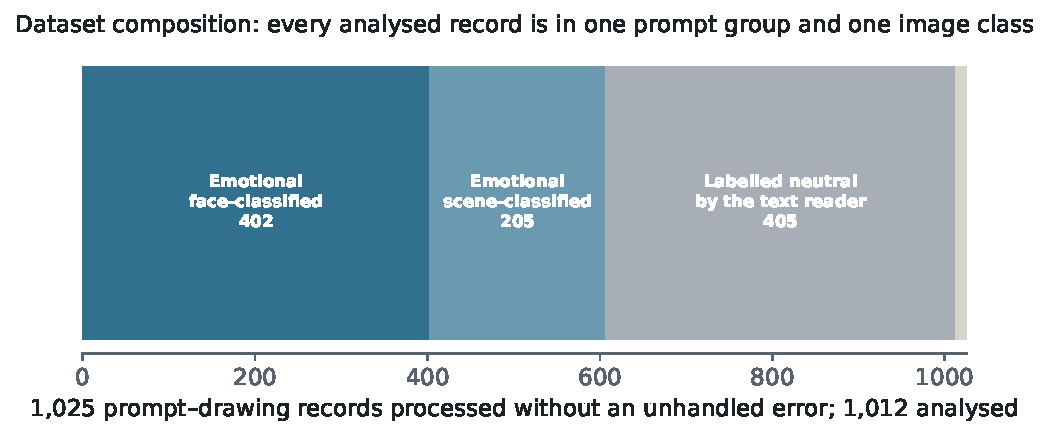
\includegraphics[width=\textwidth]{fig5_dataset}
\caption{Composition of the corpus: \nTotal\ records processed, \nPretest\ pre-festival developer tests excluded, \nAnalysed\ analysed. Every analysed record belongs to exactly one prompt group (emotional / neutral-labelled) and one image class (face-classified / scene-classified); the groups are groupings, not exclusions.}
\label{fig:dataset}
\end{figure}

\section{Data pre-processing}
\label{sec:method-preprocessing}

\subsection{Loading and pre-test removal}
% GUIDANCE: emoviz/data.py unifies three filename schemes and recovers embedded creation timestamps;
% \nPretest\ records with ids 1--13 predate the festival (developer tests) and are excluded from
% analysis but still processed, so the pipeline's completion figure covers all \nTotal.

\subsection{Prompt groups}
% GUIDANCE: dedup\_key is an integer group index computed from the ORIGINAL prompt text (stripped,
% case-folded) BEFORE redaction, so redaction can never merge two different prompts into one group.
% \nDistinct\ groups; \nGroups\ groups hold two or more records (\nGroupRecords\ records). Every
% resampling and permutation in Section~\ref{sec:method-inference} clusters on this key.
% Note the one quirk audits.py found: the key is case-insensitive but the prompt reader saw the
% original case, so a handful of groups mix readings (e.g. "Ok" and "ok"); this does not change any
% count and is reported for completeness.

\subsection{Name redaction}
% GUIDANCE: Describe as data pre-processing, per supervisor direction: names of private individuals
% are replaced by a placeholder at LOAD time; the files on disk are never modified; illness and grief
% content is kept because it is not identifying on its own and is essential to the analysis.
% Three documented stages: DETECT (high recall by design because most prompts are lower case:
% an NLTK given-name gazetteer of 7,944 names \cite{bird2009natural}, mid-sentence capitalisation
% against a 236k-word dictionary, and naming phrases such as "called X"); REVIEW (every candidate
% carries a recorded keep/redact decision with a reason, scoped to the record it was reviewed in, so
% "Jack Frost" and "woolly mammoth" survive; the audit fails if any candidate is unreviewed);
% APPLY (per record). Eight records are affected. Inertness: re-reading the redacted prompts moves
% no GoEmotions probability by more than 0.012 and changes no top-1 family; two records reduce to
% the bare placeholder and are treated separately in the control audit (Section~\ref{sec:method-audits}).
% The decision table travels with the dataset, not with the code.

\section{The pipeline}
\label{sec:method-pipeline}

\subsection{Prompt reader}
% GUIDANCE: GoEmotions \cite{demszky2020goemotions} (SamLowe/roberta-base-go\_emotions, about 125M
% parameters) returns 28 probabilities; they are summed into seven families by the grouping proposed
% with the dataset (Appendix~\ref{app:instruments}), normalised, and the top-3 kept. Rejected: zero-shot
% NLI on the prompts (a third of prompts collapsed to "surprise"); a hand lexicon (the v1 rule).
% An emotional prompt is one whose top-1 family is not neutral (\nEmotional\ of \nAnalysed).

\subsection{Describer}
% GUIDANCE: BLIP-VQA \cite{li2022blip} (Salesforce/blip-vqa-base, about 385M parameters) answers the
% five fixed questions in Appendix~\ref{app:instruments}: facial expression, action, posture, number of
% people, what is in the picture. The word "emotion" appears in none of them. Answers are cached per
% record, which is what makes the ablation possible without re-running the vision model.
% Rejected (with evidence in RESULTS\_describe\_extract.md): a 3B vision--language model that thrashed
% into swap on a 16 GB laptop for 4 h 45 min with zero progress; a plain caption, whose NLI reading
% collapsed to one family.

\subsection{Description template and image reader}
% GUIDANCE: The five answers are composed into one neutral sentence (template in
% Appendix~\ref{app:instruments}); BART-MNLI \cite{lewis2020bart, williams2018broad}
% (facebook/bart-large-mnli, about 407M parameters) scores each family as a hypothesis
% "This scene conveys \{family\}." by entailment \cite{yin2019benchmarking}; the top-3 is kept.
% Say plainly that the template asserts a person and an expression for every drawing, including
% those where the describer reports no people — the consequence is measured in
% Section~\ref{sec:results-describer} and the ablation. Rejected: GoEmotions on the description
% (collapsed to neutral above 0.95).

\subsection{Face and scene classes}
% GUIDANCE: face-classified = the describer reports at least one person AND its expression answer
% contains a word from the documented list in Appendix~\ref{app:instruments} (token match, so
% "man is smiling" counts); scene-classified otherwise. \nFaceAll\ / \nSceneAll\ over all analysed
% records; \nFaceEmo\ / \nSceneEmo\ within the emotional prompts. State the circularity now: the
% class is defined from the same description the image reader reads.

\section{The similarity ladder}
\label{sec:method-measures}
% GUIDANCE: Introduce the notation, then one short paragraph per measure explaining what it rewards
% and what it ignores. Write around the equations; do not restate them in words.

Let each reader return a top-3 list $T = \{(\ell_i, s_i)\}_{i=1}^{3}$ of families $\ell_i \in \mathcal{F}$ with scores $s_i$, where $\mathcal{F} = \{\text{joy}, \text{sadness}, \text{anger}, \text{fear}, \text{surprise}, \text{disgust}, \text{neutral}\}$. Write $P$ for the prompt reader's list and $Q$ for the image reader's, and $\operatorname{top}(T) = \ell_1$ for the top-1 family. Each family has a fixed centroid $c_\ell = (v_\ell, a_\ell)$ on the valence--arousal circumplex (Appendix~\ref{app:instruments}).

\paragraph{Valence--arousal similarity.} The score-weighted centroid of a reading and the similarity between two readings are
\begin{equation}
\mathbf{v}(T) = \frac{\sum_i s_i\, c_{\ell_i}}{\sum_i s_i}, \qquad
S_{\mathrm{VA}}(P, Q) = 1 - \frac{1}{\sqrt{2}}\,\Bigl\|\Bigl(\tfrac{v_P + 1}{2} - \tfrac{v_Q + 1}{2},\; a_P - a_Q\Bigr)\Bigr\|_2 ,
\label{eq:va}
\end{equation}
where $(v_P, a_P) = \mathbf{v}(P)$ and likewise for $Q$. Valence is rescaled to $[0,1]$ so both axes have unit range. Over the seven centroids the smallest attainable value is $0.412$ (joy against sadness), and randomly paired records average about \FullNeuVaNull; this floor is why the measure is never quoted without its null.

\paragraph{Top-3 soft overlap.} Each side is first normalised to a distribution over its own three families, $\tilde{p}_\ell = s_\ell / \sum_j s_j$, so the prompt reader's multi-label scale and the image reader's softmax scale are comparable; the overlap is the sum of per-family minima,
\begin{equation}
S_{\mathrm{ovl}}(P, Q) = \sum_{\ell \in \mathcal{F}} \min\bigl(\tilde{p}_\ell,\; \tilde{q}_\ell\bigr) \in [0, 1],
\label{eq:overlap}
\end{equation}
which equals one only when the two distributions coincide.

\paragraph{Family agreement.} Over a set of $n$ records,
\begin{equation}
A_{\mathrm{fam}} = \frac{1}{n} \sum_{i=1}^{n} \mathbb{1}\bigl[\operatorname{top}(P_i) = \operatorname{top}(Q_i)\bigr].
\label{eq:family}
\end{equation}

\paragraph{Valence-sign agreement.} With $\sigma(\ell) \in \{+, -, 0\}$ the sign of a family ($+$ for joy; $-$ for sadness, anger, fear, disgust; $0$ for surprise and neutral),
\begin{equation}
A_{\mathrm{sign}} = \frac{\sum_{i} \mathbb{1}\bigl[\sigma(\operatorname{top} P_i) \neq 0 \;\wedge\; \sigma(\operatorname{top} P_i) = \sigma(\operatorname{top} Q_i)\bigr]}{\sum_{i} \mathbb{1}\bigl[\sigma(\operatorname{top} P_i) \neq 0\bigr]} ,
\label{eq:sign}
\end{equation}
so records whose prompt family has no sign are excluded from the denominator; the denominator is reported with every value (for example \FullEmoNSign\ of the \FullEmoN\ emotional prompts).

\section{The random-pairing null}
\label{sec:method-null}
% GUIDANCE: Why a null: the measures do not start at zero (Eq.~\ref{eq:va}'s floor; the family
% marginals in Table~\ref{tab:families} make "joy" agreement likely by chance). The null is the
% exchangeability hypothesis that the image reading is unrelated to the prompt \cite{good2005permutation}.
% Note that with K = \nullShuffles\ re-pairings the null sd is itself an estimate: across seeds 1--5 the
% headline z moves between \ZSeedMin\ and \ZSeedMax, so z orders effects, it is not a precise
% probability. Then degenerate nulls, detected automatically from the null's spread.

For a subset of $n$ records and a measure $m$, draw $K$ random permutations $\pi_k$ of the image readings and compute $m_k = m\bigl(\{(P_i, Q_{\pi_k(i)})\}_{i=1}^{n}\bigr)$. With $\hat\mu = \frac{1}{K}\sum_k m_k$ and $\hat\sigma$ the standard deviation of $\{m_k\}$,
\begin{equation}
z = \frac{m_{\mathrm{obs}} - \hat\mu}{\hat\sigma}, \qquad K = \nullShuffles,\ \text{seed}\ \nullSeed .
\label{eq:z}
\end{equation}
A null is \emph{degenerate} when $\hat\sigma = 0$: this happens for family agreement when every prompt in the subset shares one top-1 family, and for valence-sign agreement when every prompt shares one sign, because permuting the image side then cannot change the score. The analysis detects this from the null itself and prints no $z$ for such cells.

\section{Inference}
\label{sec:method-inference}
% GUIDANCE: Explain why records are not independent (\nRepeats\ repeats) and that every interval and
% test therefore clusters on the prompt group \cite{cameron2008bootstrap}. One paragraph each.

\paragraph{Clustered bootstrap confidence intervals.} Let $\mathcal{G}$ be the set of prompt groups in a subset. For $b = 1, \dots, B$ draw $|\mathcal{G}|$ groups with replacement, pool their records, and recompute the measure; the 95\% interval is the 2.5th and 97.5th percentiles of the $B$ values \cite{efron1993introduction}, with $B = \DiffDraws$ and seed \nullSeed.

\paragraph{Clustered permutation test of the face/scene difference.} Under the null that the image class is unrelated to agreement, the face/scene labels are exchangeable across prompt groups. The labels are permuted across groups $P$ times and the difference in agreement recomputed; the two-sided $p$-value uses the estimator of \cite{north2002note},
\begin{equation}
p = \frac{k + 1}{P + 1}, \qquad k = \#\{\text{permuted differences at least as extreme as the observed}\},
\label{eq:permp}
\end{equation}
so the smallest reportable value with $P = \DiffDraws$ is $10^{-4}$.

\paragraph{Cohen's kappa.} For comparability with other studies, family agreement is also reported as
\begin{equation}
\kappa = \frac{p_o - p_e}{1 - p_e},
\label{eq:kappa}
\end{equation}
with $p_o$ the observed top-1 agreement and $p_e$ the agreement expected from the two readers' family marginals \cite{cohen1960coefficient}, interpreted with the bands of \cite{landis1977measurement}; intervals by the clustered bootstrap above.

\paragraph{Multiple comparisons.} The analysis prints \HolmM\ non-degenerate $z$-scores. Each is converted to a two-sided $p$ by the normal approximation and the family is controlled with the Holm--Bonferroni step-down procedure \cite{holm1979simple}: order $p_{(1)} \le \dots \le p_{(m)}$ and reject while $p_{(i)} \le \alpha / (m - i + 1)$, $\alpha = 0.05$.

\paragraph{Paired comparison of two image readers.} On the same records each reader either agrees with the prompt reader or does not. With $b$ the records only the first reader agrees on and $c$ only the second, McNemar's exact binomial test \cite{mcnemar1947note} on $(b, c)$ treats records as independent and is therefore optimistic here; the clustered version flips the sign of each prompt group's summed difference as a block (\McClusterDraws\ draws) and the clustered bootstrap gives the interval on the difference in rates.

\paragraph{Wilson intervals.} Proportions from the single-coder check use the Wilson score interval \cite{wilson1927probable}, which behaves at small $n$ and near 0 and 1.

\section{Analyses}
\label{sec:method-analyses}
% GUIDANCE: One paragraph per analysis, in the order the results are reported. Name the script.
%   Splits (analysis\_final.py): emotional / neutral-labelled prompts; face / scene within emotional;
%     positive / negative valence (VA only, the others are degenerate); all against the null of Eq.~\ref{eq:z}.
%   Distinct-prompt robustness: the same table on the first occurrence of each prompt (\nDistinct\ records).
%   Face/scene difference (significance.py): clustered bootstrap CI and clustered permutation test.
%   Specificity check: neutral-labelled prompts should sit at their null; only VA is informative there.
%   Method comparison (method\_comparison.py): the SAME prompt reader, subset, measures and re-pairings,
%     varying only the image reader (describe-then-extract vs direct CLIP zero-shot \cite{radford2021learning,
%     ilharco2021openclip}); paired tests as above. State that the earlier v1 comparison used a different
%     prompt reader, subset and overlap formula and is kept only as a record (Table~\ref{tab:methodvone}).
%   Consistency (data\_audit\_consistency.py): defined below, with its permutation null.
%   Control audit (audits.py): a fixed \CtrlLexicon-word affect lexicon over the \CtrlN\ neutral-labelled
%     prompts; the two placeholder-only records; the specificity check re-run on the cleaned control.
%   Describer audit (audits.py): people count crossed with expression word; the copy rate defined below.
%   Error taxonomy (error\_taxonomy.py): every emotional record where both readers score at least 0.8 and
%     disagree on family, each drawing inspected and assigned one of six failure modes.
%   Ablation (ablate\_nli.py): rebuild each description from the cached answers with one clause removed
%     (expression, action, posture, people, scene) or the expression fixed to "unclear"; re-run only the
%     NLI stage; recompute the ladder and nulls with identical code.
%   Human check (human\_check.py): a fixed, stratified 120-drawing sample coded by one coder blind to
%     prompt and model output for person present, readable face, valence and family; describer and reader
%     scored against the codes with Wilson intervals; the face/scene contrast re-run on the coder's split.

\paragraph{Consistency across repeated prompts.} For a prompt group $g$ with $n_g \ge 2$ records and image top-1 families $\{\operatorname{top}(Q_i)\}_{i \in g}$, the modal fraction is $c_g = \max_{\ell} n_{g,\ell} / n_g$, and the consistency is the mean $C = \frac{1}{|\mathcal{G}_{\ge 2}|} \sum_g c_g$ over the \nGroups\ groups. Because \nPairGroups\ groups are pairs, $c_g$ cannot fall below $0.5$ for them, so $C$ is read against a permutation null that shuffles the image top-1 families across all \nAnalysed\ analysed records and re-cuts them into the same groups (\ConsDraws\ draws). The count of fully consistent groups ($c_g = 1$) is treated the same way. This bounds the reproducibility of the whole prompt-to-reading chain; it does not isolate the generator, whose parameters were not recorded.

\paragraph{Copy rate.} Where the describer's expression answer is a single word that names an emotion (strict: happy, sad, angry, \dots; \DescBareStrictN\ records) or a facial action with an implied family (broad: smile, crying, \dots; \DescBareBroadN\ records), the copy rate is the share of those records in which the image reader's top-1 family equals the family the word implies. It measures how much the "separate" extraction stage adds beyond the describer's own word.

\section{The demonstrator}
\label{sec:method-demo}
% GUIDANCE: A local Flask application that runs the real pipeline on any of the \nAnalysed\ records
% or an uploaded image, shows the five answers and the description, both readings, and the ladder
% against the SAME null as the analysis (computed at start-up from the same result files). Design
% choices to state: the valence--arousal axis starts at its floor and shades the middle half of random
% pairings; the verdict leads with valence sign and family; nothing a visitor types or uploads is
% stored. It is a testing and communication tool, not a data-collection tool.

\section{Reproducibility and testing}
\label{sec:method-repro}
% GUIDANCE: Pinned environment (requirements.txt), seeded randomness, cached model outputs so every
% analysis re-runs in seconds, a frozen direct-CLIP baseline file, and one metrics module shared by
% every script so definitions cannot drift. Two layers of tests: test.sh (smoke checks — environment,
% data integrity, every script exits 0, a live three-image pipeline run, the redaction audit) and
% test\_numeric.py (every headline value pinned to the JSON that produces it, plus unit tests of the
% measures: the 0.412 floor, symmetry, overlap bounds). Figures and every number in this document are
% generated from the same JSON (make\_figures.py, export\_tex.py). Say what the tests do NOT do: none
% validates a model answer against a human label — that is what the human check is for.
% Appendix~\ref{app:repro} lists the files and the run order.
